% !TeX program = xelatex
% !TeX root = guide.tex
\documentclass[11pt,a4paper]{article}

\usepackage{iftex}
\ifPDFTeX
  \usepackage[T1]{fontenc}
  \usepackage[utf8]{inputenc}
  \usepackage{lmodern}
\fi
\usepackage[a4paper,margin=20mm]{geometry}
\usepackage{microtype}
\usepackage[table]{xcolor}
\usepackage{graphicx}
\usepackage{booktabs}
\usepackage{array}
\usepackage{tabularx}
\usepackage{longtable}
\usepackage{fancyhdr}
\usepackage{hyperref}
\usepackage{tikz}

\usetikzlibrary{arrows.meta,backgrounds,calc,fit,positioning,shapes.geometric,shapes.misc}

\definecolor{TitleBlue}{HTML}{173F5F}
\definecolor{AccentTeal}{HTML}{1F7A8C}
\definecolor{AccentGold}{HTML}{E0A458}
\definecolor{SoftSand}{HTML}{F5EFE7}
\definecolor{SoftBlue}{HTML}{EAF4F4}
\definecolor{SoftGray}{HTML}{F3F5F7}
\definecolor{Ink}{HTML}{24323F}
\definecolor{LightLine}{HTML}{C8D1D9}

\hypersetup{
  colorlinks=true,
  linkcolor=TitleBlue,
  urlcolor=AccentTeal,
  pdftitle={kubernetes-minikube repository guide},
  pdfauthor={Codex},
  pdfsubject={Repository explanation and execution guide}
}

\pagestyle{fancy}
\fancyhf{}
\fancyhead[L]{\sffamily\small kubernetes-minikube guide}
\fancyhead[R]{\sffamily\small \today}
\fancyfoot[C]{\sffamily\small \thepage}
\setlength{\headheight}{14pt}
\setlength{\parindent}{0pt}
\setlength{\parskip}{6pt}
\renewcommand{\familydefault}{\rmdefault}
\renewcommand{\arraystretch}{1.2}

\newcolumntype{Y}{>{\raggedright\arraybackslash}X}
\newcolumntype{P}[1]{>{\raggedright\arraybackslash}p{#1}}
\newcommand{\repo}{\texttt{kubernetes-minikube}}
\newcommand{\pathitem}[1]{\texorpdfstring{\nolinkurl{#1}}{#1}}
\newcommand{\cmd}[1]{\texttt{#1}}
\Urlmuskip=0mu plus 1mu

\begin{document}
\hypersetup{pageanchor=false}

\begin{titlepage}
\thispagestyle{empty}
\begin{tikzpicture}[remember picture,overlay]
  \fill[SoftSand] (current page.south west) rectangle (current page.north east);
  \fill[TitleBlue] (current page.north west) rectangle ([yshift=-4.2cm]current page.north east);
  \fill[AccentGold] ([xshift=-5.2cm,yshift=-5.2cm]current page.north east) circle (2.5cm);
  \fill[AccentTeal!88] ([xshift=3.8cm,yshift=3cm]current page.south west) circle (2.9cm);
  \node[
    draw=white,
    line width=1.2pt,
    rounded corners=14pt,
    text=white,
    align=left,
    anchor=north,
    inner xsep=16pt,
    inner ysep=14pt,
    text width=12.6cm
  ] at ([yshift=-1.05cm]current page.north) {%
    {\sffamily\fontsize{24}{28}\selectfont Repository Structure\\and Execution Guide\par}
    \vspace{3mm}
    {\sffamily\large for \repo\par}
  };
\end{tikzpicture}

\vspace*{4.95cm}
{\large This document explains what the repository contains, how the pieces fit together, and what you should do step by step to run, extend, and validate it.\par}

\vfill

\begin{tabularx}{\linewidth}{@{}p{0.22\linewidth}Y@{}}
\rowcolor{white}
\textbf{Repository} & \repo \\
\rowcolor{SoftBlue}
\textbf{Main goal} & Learn the path from a local Spring Boot service to a containerized application exposed through Minikube with Deployment, Service, LoadBalancer, and Ingress resources. \\
\rowcolor{white}
\textbf{Key payload} & A small Java web service, a multi-stage Docker build, Kubernetes manifests, and an instructional README. \\
\rowcolor{SoftBlue}
\textbf{Expected outcome} & You can build the image, publish or load it, deploy it on Minikube, expose it with the desired network primitive, and understand why each layer exists. \\
\end{tabularx}

\vspace{1cm}
{\sffamily\large \today\par}
\end{titlepage}
\hypersetup{pageanchor=true}

\tableofcontents
\newpage

\section{What this repository is}

\repo{} is a compact teaching repository. It is not a large production platform and it is not a full microservice system. Instead, it is a minimal but complete chain that demonstrates four linked concerns:

\begin{enumerate}
\item building a Java web service,
\item packaging that service into a Docker image,
\item running the image inside Kubernetes on Minikube,
\item exposing the application through progressively more advanced Kubernetes networking resources.
\end{enumerate}

The application itself is intentionally small. The business logic is a single HTTP endpoint that returns the string \cmd{Hello}. That simplicity is useful because it keeps the focus on containerization and orchestration instead of application complexity.

\subsection{The core learning path}

The repository is designed so that each stage adds one new layer:

\begin{enumerate}
\item run the service directly as a container,
\item manage the container as a Kubernetes Deployment,
\item make it reachable through a Service,
\item experiment with Service types such as NodePort and LoadBalancer,
\item route incoming HTTP traffic through an Ingress rule.
\end{enumerate}

If you understand that chain, you understand the educational purpose of the repository.

\section{Repository map}

Figure \ref{fig:repomap} shows the physical structure of the repository. The most important split is between the application source in \pathitem{MyService/} and the Kubernetes manifests stored at the repository root.

\begin{figure}[ht]
\centering
\begin{tikzpicture}[
  font=\sffamily\small,
  node distance=9mm,
  summary/.style={draw=TitleBlue, rounded corners=6pt, fill=white, inner sep=7pt, text width=11.0cm, align=left},
  repo/.style={draw=TitleBlue, rounded corners=6pt, fill=SoftSand, inner sep=8pt, text width=9.2cm, align=center}
]
  \node[repo] (root) {\textbf{kubernetes-minikube}\\A teaching repository that combines a tiny Java service with Docker packaging and Kubernetes manifests for Minikube exercises.};

  \node[summary, below=of root] (rootfiles) {\textbf{Repository root files}\\
  \textbullet~\pathitem{README.md}: guided walkthrough\\
  \textbullet~\pathitem{myservice-deployment.yml}: pod template and image\\
  \textbullet~\pathitem{myservice-service.yml}: NodePort exposure\\
  \textbullet~\pathitem{myservice-loadbalancing-service.yml}: LoadBalancer variant\\
  \textbullet~\pathitem{ingress.yml}: host-based HTTP routing\\
  \textbullet~\pathitem{.gitignore}: local artifact filtering};

  \node[summary, below=of rootfiles, fill=SoftBlue] (appfiles) {\textbf{Application payload in \pathitem{MyService/}}\\
  \textbullet~Spring Boot source code\\
  \textbullet~\pathitem{src/main/.../MyServiceRest.java}: \cmd{GET /}\\
  \textbullet~\pathitem{build.gradle}: Java 21 and Spring web\\
  \textbullet~\pathitem{Dockerfile}: multi-stage image build\\
  \textbullet~Gradle wrapper and smoke test};

  \draw[-{Latex[length=3mm]}, thick, TitleBlue] (root.south) -- (rootfiles.north);
  \draw[-{Latex[length=3mm]}, thick, TitleBlue] (rootfiles.south) -- node[right, font=\sffamily\scriptsize]{deploys and exposes} (appfiles.north);
\end{tikzpicture}
\caption{Repository structure and the role of each top-level asset.}
\label{fig:repomap}
\end{figure}

\subsection{Files you are most likely to touch}

\small
\begin{longtable}{@{}P{0.38\linewidth}P{0.24\linewidth}P{0.30\linewidth}@{}}
\toprule
\textbf{Path} & \textbf{Why it exists} & \textbf{When you edit it} \\
\midrule
\endhead
\pathitem{MyService/.../MyServiceRest.java} & Exposes the actual HTTP endpoint. & When you change application behavior or add routes. \\
\pathitem{MyService/Dockerfile} & Builds the runnable container image. & When the build process, base image, or runtime image changes. \\
\pathitem{myservice-deployment.yml} & Declares the pod template and container image used by Kubernetes. & When you change image name, tag, replicas, or pod settings. \\
\pathitem{myservice-service.yml} & Exposes the deployment through a fixed NodePort. & When you want outside access from Minikube using a port on the node. \\
\pathitem{myservice-loadbalancing-service.yml} & Provides an alternative Service definition using type LoadBalancer. & When you want to test a load-balanced exposure pattern. \\
\pathitem{ingress.yml} & Adds host-based HTTP routing on top of the service. & When you want friendly URLs or multiple routes through one entry point. \\
\pathitem{README.md} & Walkthrough for learners. & When you want to refine the instructions or update command examples. \\
\bottomrule
\end{longtable}
\normalsize

\section{How the runtime pieces fit together}

The repository is easiest to understand as a traffic path. A browser request does not talk to the Java code directly once Kubernetes is involved. It crosses a sequence of layers. Figure \ref{fig:runtime} shows that path.

\begin{figure}[ht]
\centering
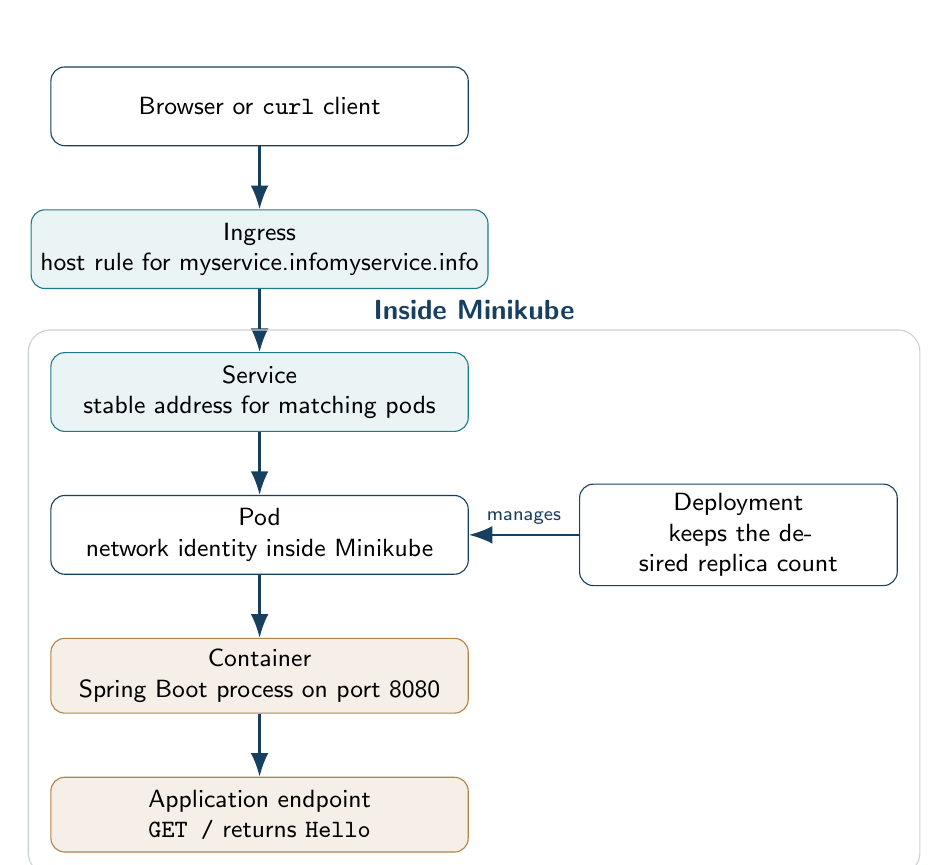
\begin{tikzpicture}[
  font=\sffamily\small,
  node distance=8mm and 14mm,
  flow/.style={draw=TitleBlue, rounded corners=5pt, fill=white, minimum width=5.3cm, minimum height=1.0cm, align=center},
  accent/.style={draw=AccentTeal, rounded corners=5pt, fill=SoftBlue, minimum width=5.3cm, minimum height=1.0cm, align=center},
  innerbox/.style={draw=AccentGold!80!black, rounded corners=5pt, fill=SoftSand, minimum width=5.3cm, minimum height=0.95cm, align=center}
]
  \node[flow] (browser) {Browser or \cmd{curl} client};
  \node[accent, below=of browser] (ingress) {Ingress\\host rule for \pathitem{myservice.info}};
  \node[accent, below=of ingress] (service) {Service\\stable address for matching pods};
  \node[flow, below=of service] (pod) {Pod\\network identity inside Minikube};
  \node[innerbox, below=of pod] (container) {Container\\Spring Boot process on port 8080};
  \node[innerbox, below=of container] (rest) {Application endpoint\\\cmd{GET /} returns \cmd{Hello}};
  \node[flow, right=of pod, text width=3.8cm, minimum width=3.9cm] (deployment) {Deployment\\keeps the desired replica count};

  \draw[-{Latex[length=3mm]}, thick, TitleBlue] (browser) -- (ingress);
  \draw[-{Latex[length=3mm]}, thick, TitleBlue] (ingress) -- (service);
  \draw[-{Latex[length=3mm]}, thick, TitleBlue] (service) -- (pod);
  \draw[-{Latex[length=3mm]}, thick, TitleBlue] (pod) -- (container);
  \draw[-{Latex[length=3mm]}, thick, TitleBlue] (container) -- (rest);
  \draw[-{Latex[length=3mm]}, thick, TitleBlue] (deployment.west) -- node[above, font=\sffamily\scriptsize]{manages} (pod.east);

  \node[draw=LightLine, rounded corners=8pt, fit=(service)(pod)(container)(rest)(deployment), inner sep=8pt, label={[font=\sffamily\bfseries, text=TitleBlue]above:Inside Minikube}] {};
\end{tikzpicture}
\caption{Logical request path from the client to the Spring Boot endpoint.}
\label{fig:runtime}
\end{figure}

\subsection{What each layer contributes}

\begin{itemize}
\item The \textbf{container} packages the application and its runtime environment.
\item The \textbf{pod} is the smallest deployable unit in Kubernetes and gives the container a cluster network identity.
\item The \textbf{deployment} keeps the desired number of pod replicas running and handles updates.
\item The \textbf{service} gives a stable access point even if pod IP addresses change.
\item The \textbf{ingress} adds human-friendly routing and external HTTP entry behavior.
\end{itemize}

This is why the repository has separate files for deployment, service, and ingress. They do different jobs even though they point to the same application.

\section{What is inside the application}

The Java application is deliberately minimal:

\begin{itemize}
\item \pathitem{MyServiceApplication.java} starts the Spring Boot application.
\item \pathitem{MyServiceRest.java} defines one REST endpoint on \cmd{/}.
\item \pathitem{application.properties} is currently empty, which means the default Spring Boot web settings are used.
\item \pathitem{MyserviceApplicationTests.java} only checks that the Spring context starts successfully.
\end{itemize}

This matters because the repository is mostly about infrastructure. The app is just a dependable target to deploy.

\subsection{What the Dockerfile does}

The Dockerfile uses a two-stage build:

\begin{enumerate}
\item a \textbf{build stage} based on \cmd{gradle:8.5-jdk21} compiles the project and creates the JAR,
\item a \textbf{runtime stage} based on \cmd{eclipse-temurin:21-jre} copies only the built JAR and launches it with \cmd{java -jar app.jar}.
\end{enumerate}

That design keeps the final runtime image smaller than a single-stage build because Gradle and the build toolchain do not need to remain in the production image.

\section{Pedagogical progression of the repository}

The repository is intentionally layered. Each new exercise introduces more Kubernetes surface area. Figure \ref{fig:plot} visualizes that progression as the number of repository-managed platform resources you are directly dealing with at each step.

\begin{figure}[ht]
\centering
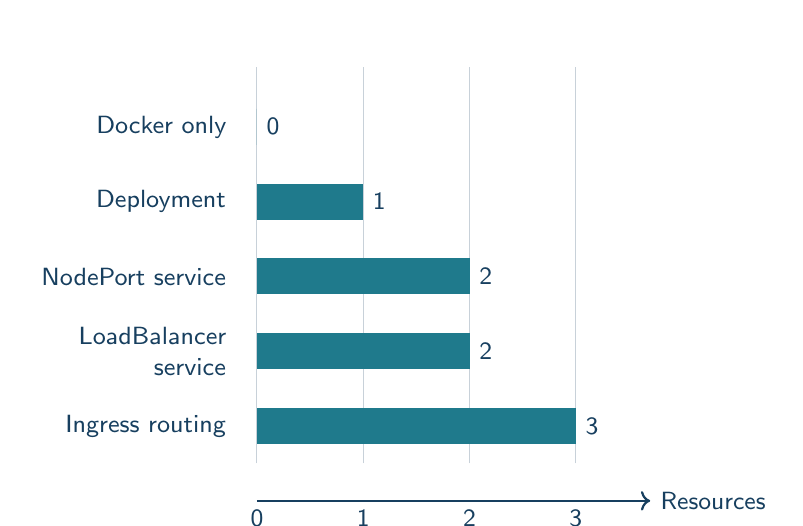
\begin{tikzpicture}[font=\sffamily\small, x=1.35cm, y=0.95cm]
  \draw[->, thick, TitleBlue] (1.5,0) -- (5.2,0) node[right] {Resources};
  \foreach \x in {0,1,2,3} {
    \draw[LightLine] ({1.5+\x},0.5) -- ({1.5+\x},5.8);
    \node[below, text=TitleBlue] at ({1.5+\x},0) {\x};
  }

  \foreach \y/\label/\value in {
    5/Docker only/0,
    4/Deployment/1,
    3/NodePort service/2,
    2/LoadBalancer service/2,
    1/Ingress routing/3
  } {
    \node[anchor=east, align=right, text width=2.4cm, text=TitleBlue] at (1.3,\y) {\label};
    \fill[AccentTeal] (1.5,\y-0.24) rectangle ({1.5+\value},\y+0.24);
    \node[TitleBlue, right] at ({1.5+\value},\y) {\value};
  }
\end{tikzpicture}
\caption{Conceptual progression through the repository. Docker alone manages no Kubernetes resource. Deployment, Service, and Ingress are added step by step.}
\label{fig:plot}
\end{figure}

This plot explains the structure of the repository better than the file list alone: the repository is a staircase from local container execution toward richer cluster networking.

\section{What you must do}

If your goal is to learn the repository in a useful order, the following sequence is the most direct path.

\subsection{Phase 1: Prepare the environment}

\begin{enumerate}
\item Install Docker Desktop or another Docker runtime.
\item Install Minikube.
\item Install \cmd{kubectl}.
\item Start the cluster with \cmd{minikube start}.
\item Confirm the cluster is reachable with \cmd{kubectl get nodes}.
\end{enumerate}

\subsection{Phase 2: Understand the real project paths}

There is one detail you should not miss: use \pathitem{MyService/}, not \pathitem{myservice/}. The repository on disk uses a capital \texttt{M} and \texttt{S}, so build commands should be run from that exact path.

\subsection{Phase 3: Build and test the container locally}

Work from \pathitem{MyService/}. The minimal validation loop is:

\begin{enumerate}
\item build the image,
\item run the container,
\item open the service at \cmd{http://localhost:4000},
\item verify that the response body is \cmd{Hello}.
\end{enumerate}

This step proves that the application itself works before Kubernetes enters the picture.

\subsection{Phase 4: Decide how Minikube will get the image}

You have two valid strategies:

\begin{itemize}
\item \textbf{Push to a registry}: build an image such as \cmd{your-dockerhub-id/myservice:1} and push it, then reference that tag in \pathitem{myservice-deployment.yml}.
\item \textbf{Load locally into Minikube}: build the image locally and load it into Minikube, then point the deployment to that same tag.
\end{itemize}

Right now the deployment manifest references \cmd{efrei/myservice:1}. That means the cluster will pull that public image unless you replace the \cmd{image:} field.

\subsection{Phase 5: Deploy the application}

The repository workflow after image preparation is:

\begin{enumerate}
\item update the deployment image if you want to use your own build,
\item apply \pathitem{myservice-deployment.yml},
\item wait for the pod to become \cmd{Running},
\item inspect pods with \cmd{kubectl get pods},
\item inspect the deployment with \cmd{kubectl get deployments}.
\end{enumerate}

\subsection{Phase 6: Expose it with one service style at a time}

The repository contains two alternative Service definitions that both use the name \cmd{myservice}:

\begin{itemize}
\item \pathitem{myservice-service.yml} creates a \textbf{NodePort} service.
\item \pathitem{myservice-loadbalancing-service.yml} creates a \textbf{LoadBalancer} service.
\end{itemize}

Treat them as alternatives, not as two independent services to keep at the same time. In practice, the normal learning order is:

\begin{enumerate}
\item start with \pathitem{myservice-service.yml},
\item test access with \cmd{minikube service myservice --url},
\item then switch to the LoadBalancer variant only when you want to learn that exposure style.
\end{enumerate}

\subsection{Phase 7: Add ingress only after the service works}

The Ingress rule in \pathitem{ingress.yml} expects a backend service named \cmd{myservice} on port \cmd{8080}. Therefore:

\begin{enumerate}
\item enable ingress support with \cmd{minikube addons enable ingress},
\item make sure the service already works,
\item apply \pathitem{ingress.yml},
\item map the hostname \cmd{myservice.info} to the Minikube address as required by your operating system,
\item test the route through the hostname rather than by raw port number.
\end{enumerate}

\subsection{Phase 8: Learn the scaling command}

Once the deployment is stable, scale it:

\begin{center}
\cmd{kubectl scale --replicas=2 deployment/myservice}
\end{center}

Then check that multiple pods are running. This is the first moment where the value of the Service abstraction becomes obvious: the Service name stays the same even when the backing pods multiply or rotate.

\section{Deep dive into the manifest files}

\subsection{\pathitem{myservice-deployment.yml}}

This file declares:

\begin{itemize}
\item \cmd{kind: Deployment},
\item one replica by default,
\item a selector on the label \cmd{app: myservice},
\item a pod template using the same label,
\item a single container named \cmd{myservice},
\item the image \cmd{efrei/myservice:1},
\item \cmd{imagePullPolicy: IfNotPresent}.
\end{itemize}

The labels are important because the Service selectors rely on them. If you rename labels in the deployment, you must keep the selectors in the service definitions aligned.

\subsection{\pathitem{myservice-service.yml}}

This file exposes the app with:

\begin{itemize}
\item \cmd{kind: Service},
\item \cmd{type: NodePort},
\item cluster port \cmd{8080},
\item target container port \cmd{8080},
\item fixed node port \cmd{31280}.
\end{itemize}

It is the most direct way to reach the app from outside the cluster during Minikube exercises.

\subsection{\pathitem{myservice-loadbalancing-service.yml}}

This file is another Service resource with the same selector but a different type:

\begin{itemize}
\item \cmd{type: LoadBalancer},
\item fixed node port \cmd{30945},
\item same external service name: \cmd{myservice}.
\end{itemize}

In a full cloud environment this would request a cloud load balancer. In Minikube, external accessibility usually depends on the Minikube service command or tunnel behavior.

\subsection{\pathitem{ingress.yml}}

This file adds an HTTP route:

\begin{itemize}
\item ingress class \cmd{nginx},
\item host \cmd{myservice.info},
\item path prefix \cmd{/},
\item backend service name \cmd{myservice},
\item backend service port \cmd{8080}.
\end{itemize}

The Ingress does not replace the Service. It sits in front of the Service.

\section{Recommended working checklist}

\begin{tabularx}{\linewidth}{@{}p{0.24\linewidth}Y@{}}
\toprule
\textbf{Step} & \textbf{What to verify} \\
\midrule
Cluster up & \cmd{kubectl get nodes} shows the Minikube node in status \cmd{Ready}. \\
Image available & The image tag used in the deployment either exists in a registry or has been loaded into Minikube. \\
Deployment applied & \cmd{kubectl get deployments} shows \cmd{myservice} with available replicas. \\
Pod healthy & \cmd{kubectl get pods} shows running pods with no crash loop. \\
Service reachable & \cmd{minikube service myservice --url} opens a working route. \\
Ingress reachable & Hostname resolution points \cmd{myservice.info} to Minikube and the NGINX ingress controller is enabled. \\
Scale works & After scaling, multiple pods exist while the service entry point remains the same. \\
\bottomrule
\end{tabularx}

\section{Common mistakes to avoid}

\begin{itemize}
\item Building a new Docker image but forgetting that the deployment YAML still points to the public tag \pathitem{efrei/myservice:1}.
\item Running commands in \pathitem{myservice/} even though the actual directory is \pathitem{MyService/}.
\item Applying the Ingress before the service is working.
\item Treating the NodePort and LoadBalancer service YAML files as if they were two different services with different names.
\item Debugging ingress before checking the simpler path through \cmd{minikube service myservice --url}.
\item Assuming the pod IP is a stable external address. It is not. The Service is the stable abstraction.
\end{itemize}

\section{What this repository is not}

It is useful to state the boundaries clearly:

\begin{itemize}
\item This repository is not a production-grade Kubernetes platform.
\item It does not include CI/CD automation, Helm charts, observability, secrets management, or multi-environment overlays.
\item It does not include persistent storage or a database.
\item It is a focused educational skeleton meant to isolate the core ideas of packaging and exposing a service.
\end{itemize}

\newpage
\appendix

\section{Appendix A: Kubernetes basics from zero}

\subsection{Cluster}

A Kubernetes cluster is a group of machines running the Kubernetes control plane and workloads. In Minikube, that cluster is usually a single local node, which makes it ideal for learning.

\subsection{Node}

A node is a machine that runs pods. In a Minikube setup, you often have exactly one node. That is enough to understand the object model even if it is not a realistic production topology.

\subsection{Pod}

A pod is the smallest deployable unit in Kubernetes. It wraps one or more containers that should run together. Pods are ephemeral. If a pod dies, Kubernetes can replace it with a new one that has a different IP address.

\subsection{Deployment}

A deployment describes the desired state of a set of pods. You specify how many replicas you want and which pod template should be used. Kubernetes then works to keep reality aligned with that declaration.

\subsection{Service}

A service creates a stable network endpoint in front of one or more pods selected by labels. This solves a fundamental problem: pods come and go, but clients need a stable way to find the application.

\subsection{Ingress}

An ingress is a set of HTTP routing rules. It is useful when you want cleaner URLs, hostnames, or multiple services exposed behind one entry point. It usually depends on an ingress controller such as NGINX.

\subsection{Selector labels}

Labels are key-value tags attached to Kubernetes objects. Services use selectors to find matching pods. In this repository, \cmd{app: myservice} is the critical label that connects the deployment and the services.

\section{Appendix B: Docker basics from zero}

\subsection{Image vs container}

A Docker image is a packaged blueprint. A container is a running instance created from that blueprint. The repository teaches you to build an image first, then run it directly, and finally hand the same image concept to Kubernetes.

\subsection{Why the Dockerfile has two stages}

The build stage compiles the Spring Boot project. The runtime stage keeps only the artifact needed to execute the app. This is cleaner and more efficient than shipping the build tools in the final image.

\subsection{Port mapping}

When you run the container locally with a mapping such as \cmd{-p 4000:8080}, the left side is the host port and the right side is the container port. The application still listens on \cmd{8080} inside the container.

\section{Appendix C: First-time execution recipe}

If you only want the shortest practical route through the repository, use this sequence as a mental model:

\begin{enumerate}
\item Start Minikube.
\item Build the Docker image from \pathitem{MyService/}.
\item Choose whether to push the image or load it into Minikube.
\item Update the deployment manifest to the image tag you actually have.
\item Apply the deployment.
\item Apply the NodePort service.
\item Test the URL returned by \cmd{minikube service myservice --url}.
\item Scale to two replicas and verify that access still works.
\item Enable ingress only after the previous step is healthy.
\item Clean up the deployment and service when you are done.
\end{enumerate}

That route matches the structure and intention of the repository.

\end{document}
